\documentclass[12pt, letterpaper]{article}

% Layout
\usepackage[margin=1in]{geometry}
\usepackage{setspace}

% Math
\usepackage{amsfonts,amsmath,amssymb,amsthm}

% Tables and figures
\usepackage{booktabs}
\usepackage{float}
\usepackage{graphicx}

% References and links
\usepackage{natbib}
\usepackage[linkcolor=blue,
            colorlinks=true,
            urlcolor=blue,
            pdfstartview={XYZ null null 1.00},
            pdfpagemode=UseNone,
            citecolor={black},
            pdftitle={Always-On Probability Calibration With Multiplicative Weights}]{hyperref}
\usepackage{url}
\usepackage{xurl}

% Misc
\setlength{\parindent}{3em}

% Footnotes
\usepackage{footmisc}
\setlength{\footnotesep}{\baselineskip}
\renewcommand{\footnotelayout}{\footnotesize \onehalfspacing}
\interfootnotelinepenalty=10000

% Caption
\usepackage[
    skip            =0pt,
    labelfont       =bf,
    font            =small,
    textfont        =small,
    figurename      =Figure,
    justification   =justified,
    singlelinecheck =false,
    labelsep        =period]
{caption}

% Theorem environments
\newtheorem{theorem}{Theorem}[section]
\newtheorem{lemma}[theorem]{Lemma}
\newtheorem{proposition}[theorem]{Proposition}
\newtheorem{corollary}[theorem]{Corollary}
\theoremstyle{definition}
\newtheorem{definition}[theorem]{Definition}
\theoremstyle{remark}
\newtheorem{remark}[theorem]{Remark}

\title{Always-On Probability Calibration With Multiplicative Weights\thanks{\href{https://github.com/finite-sample/mw-calibration}{https://github.com/finite-sample/mw-calibration}.}}

\author{Gaurav Sood\thanks{Gaurav can be reached at \href{mailto:gsood07@gmail.com}{\footnotesize{\texttt{gsood07@gmail.com}}}}\vspace{.5cm}}

\date{\today}

\begin{document}

\maketitle

\begin{abstract}
We propose a solver-free, streaming approach to post-hoc probability calibration based on multiplicative-weights updates (MWU). Standard techniques (Platt scaling, isotonic regression) are trained in batch and periodically refit, creating a tradeoff between compute cost and calibration drift. MWU performs a single exponential update per bucket per batch, requiring constant time regardless of total traffic. We show that the expected calibration map is a strongly monotone operator with curvature equal to the Bernoulli variance of the calibrated predictions. This structure makes the MWU update a Robbins-Monro stochastic approximation scheme: under stationarity with diminishing step sizes, the squared calibration error converges to zero at rate $O(1/t)$, faster than the $O(1/\sqrt{T})$ rate available from standard regret analysis. Under non-stationarity with constant step size, we bound the tracking error as a function of the step size and the drift rate. Experiments on synthetic, semi-synthetic, and production-scale streams show that MWU matches the Brier score of classical calibrators, adapts faster to drift, and requires 50--60$\times$ less compute.
\end{abstract}

\section{Introduction}

Probability calibration is critical in advertising, recommendations, and risk models \citep{Niculescu05, Guo17}. The dominant post-hoc techniques, Platt scaling \citep{Platt99} and isotonic regression \citep{Zadrozny02}, are trained in batch and periodically refit. In high-velocity settings, this creates a compute-drift tradeoff: infrequent retraining leads to miscalibration, whereas frequent retraining incurs heavy CPU costs.

We recast calibration as an online root-finding problem over bucket-wise bias factors and apply multiplicative-weights updates \citep{Arora12}. The result is an always-on calibrator that adapts to drift with constant per-batch cost. Our theoretical contribution is to show that the calibration map has a monotone operator structure that makes the MWU update a well-posed stochastic approximation scheme with provable convergence guarantees. Unlike regret-based analyses, which compare cumulative loss to a fixed comparator and yield $O(1/\sqrt{T})$ rates, our approach directly analyzes the actual calibration error and yields $O(1/t)$ convergence under stationarity and explicit tracking bounds under drift.

\section{Problem Setup}
\label{sec:setup}

Given raw probabilities $p_i^{\mathrm{raw}} \in (0,1)$ and binary outcomes $y_i \in \{0,1\}$, let $b(i) \in \{1,\dots,B\}$ denote the reliability bucket for observation $i$. We seek positive bias factors $c_b > 0$ such that the calibrated probabilities
\begin{equation}
\label{eq:calibrated}
p_i^{\mathrm{cal}} = \frac{c_{b(i)} \cdot p_i^{\mathrm{raw}}}{1 - p_i^{\mathrm{raw}} + c_{b(i)} \cdot p_i^{\mathrm{raw}}}
\end{equation}
are approximately self-calibrated: within each bucket $b$, the mean calibrated probability $\tilde{r}_b = \frac{1}{n_b}\sum_{i:b(i)=b} p_i^{\mathrm{cal}}$ matches the empirical outcome rate $\hat{r}_b = \frac{1}{n_b}\sum_{i:b(i)=b} y_i$.

\begin{proposition}[Odds-ratio calibration]
\label{prop:odds}
The functional form \eqref{eq:calibrated} arises from scaling the odds of the raw prediction by $c_b$:
\[
\frac{p_i^{\mathrm{cal}}}{1-p_i^{\mathrm{cal}}} = c_{b(i)} \cdot \frac{p_i^{\mathrm{raw}}}{1-p_i^{\mathrm{raw}}}.
\]
When the raw model is Bayes-optimal under training priors and deployment differs only by class priors, the optimal $c_b$ is the ratio of deployment to training odds for each bucket. This is the standard label-shift correction \citep{saerens2002,lipton2018}.
\end{proposition}

Setting $c_b = 1$ for all $b$ recovers the original predictions. Working in log-space, define $\theta_b = \log c_b \in [\log c_{\min}, \log c_{\max}]$. The calibration problem reduces to finding the bias vector $\boldsymbol{\theta} \in \Theta = [\log c_{\min}, \log c_{\max}]^B$ from streaming data.

\section{Multiplicative-Weights Calibrator}
\label{sec:mwu}

Data arrive in batches $t = 1, \dots, T$. After observing batch $t$, we compute the per-bucket calibration error
\[
\ell_b^{(t)} = \tilde{r}_b^{(t)} - \hat{r}_b^{(t)},
\]
the difference between the mean calibrated probability and the empirical outcome rate in bucket $b$. The MWU update is
\begin{equation}
c_b^{(t+1)} = \mathrm{clip}\!\left(c_b^{(t)} \exp\!\left(-\eta_t\, \ell_b^{(t)}\right),\; c_{\min},\; c_{\max}\right),
\label{eq:mwu}
\end{equation}
or equivalently in log-space,
\begin{equation}
\theta_b^{(t+1)} = \Pi_\Theta\!\left(\theta_b^{(t)} - \eta_t\, \ell_b^{(t)}\right),
\label{eq:mwu_log}
\end{equation}
where $\Pi_\Theta$ denotes projection (clipping) onto $\Theta$. When the calibrated probability exceeds the outcome rate ($\ell_b > 0$), the bias factor decreases; when outcomes exceed predictions ($\ell_b < 0$), the bias factor increases.

If bucket $b$ receives no observations in batch $t$, we set $\ell_b^{(t)} = 0$ and leave $c_b$ unchanged. With no data, there is no signal to update the bias.

\section{Theoretical Analysis}
\label{sec:theory}

Standard analyses of MWU proceed through online regret bounds, comparing cumulative loss to a fixed comparator. This yields $O(1/\sqrt{T})$ convergence of the average excess loss but does not directly address the actual calibration error. We take a different approach: we show that the expected calibration map has a monotone operator structure that makes \eqref{eq:mwu_log} a Robbins-Monro stochastic approximation scheme. The novel contribution is identifying this structure (Lemma~\ref{lem:derivative} and Theorem~\ref{thm:monotone}); the convergence and tracking results that follow are standard consequences of strong monotonicity in the stochastic approximation literature.

\subsection{The Calibration Map Is a Strongly Monotone Operator}

Define the expected calibration map $F: \Theta \to \mathbb{R}^B$ by $F_b(\boldsymbol{\theta}) = \mathbb{E}[\tilde{r}_b(\boldsymbol{\theta})] - \mathbb{E}[\hat{r}_b]$, the expected calibration error in bucket $b$ as a function of the bias parameters.

\begin{lemma}[Derivative of the calibration map]
\label{lem:derivative}
Each component $F_b$ depends only on $\theta_b$, and its derivative is
\[
\frac{\partial F_b}{\partial \theta_b} = \mathbb{E}\!\left[\frac{1}{n_b}\sum_{i:b(i)=b} p_i^{\mathrm{cal}}(\theta_b)\bigl(1-p_i^{\mathrm{cal}}(\theta_b)\bigr)\right].
\]
\end{lemma}

\begin{proof}
Since $\hat{r}_b$ does not depend on $\boldsymbol{\theta}$, $\frac{\partial F_b}{\partial \theta_b} = \frac{\partial}{\partial \theta_b}\mathbb{E}[\tilde{r}_b]$. For a single observation with raw probability $p$ and bias factor $c = e^{\theta_b}$, the calibrated probability is $q = cp/(1-p+cp)$. Differentiating with respect to $\theta_b$:
\[
\frac{\partial q}{\partial \theta_b} = \frac{\partial q}{\partial c}\cdot c = \frac{p(1-p)}{(1-p+cp)^2}\cdot c = \frac{cp(1-p)}{(1-p+cp)^2}.
\]
Since $q = cp/(1-p+cp)$ and $1-q = (1-p)/(1-p+cp)$, the product $q(1-q) = cp(1-p)/(1-p+cp)^2$ equals the derivative. Averaging over observations in bucket $b$ and taking expectations gives the result. The Jacobian of $F$ is diagonal because bucket assignments are determined by raw probabilities, not by $\boldsymbol{\theta}$, so $\tilde{r}_b$ depends only on $\theta_b$.
\end{proof}

\begin{theorem}[Strong monotonicity of the calibration map]
\label{thm:monotone}
Let $\mu_b(\boldsymbol{\theta}) = \mathbb{E}\!\left[\frac{1}{n_b}\sum_{i:b(i)=b} q_i(1-q_i)\right]$ denote the expected average Bernoulli variance in bucket $b$, and define $\mu = \min_{b} \inf_{\boldsymbol{\theta} \in \Theta} \mu_b(\boldsymbol{\theta})$. If $\mu > 0$, then $F$ is strongly monotone on $\Theta$:
\[
\langle F(\boldsymbol{\theta}) - F(\boldsymbol{\theta}'), \boldsymbol{\theta} - \boldsymbol{\theta}' \rangle \ge \mu \|\boldsymbol{\theta} - \boldsymbol{\theta}'\|^2 \quad \text{for all } \boldsymbol{\theta}, \boldsymbol{\theta}' \in \Theta.
\]
\end{theorem}

\begin{proof}
Since $F$ has a diagonal Jacobian (Lemma~\ref{lem:derivative}), strong monotonicity holds if each diagonal entry is bounded below by $\mu$. By the mean value theorem, $F_b(\theta_b) - F_b(\theta_b') = F_b'(\tilde\theta_b)(\theta_b - \theta_b')$ for some $\tilde\theta_b$ between $\theta_b$ and $\theta_b'$. By Lemma~\ref{lem:derivative}, $F_b'(\tilde\theta_b) = \mu_b(\tilde{\boldsymbol{\theta}}) \ge \mu$. Summing over buckets:
\[
\langle F(\boldsymbol{\theta}) - F(\boldsymbol{\theta}'), \boldsymbol{\theta} - \boldsymbol{\theta}' \rangle = \sum_b F_b'(\tilde\theta_b)(\theta_b - \theta_b')^2 \ge \mu \|\boldsymbol{\theta} - \boldsymbol{\theta}'\|^2.
\]
\end{proof}

\begin{remark}
The condition $\mu > 0$ requires that no bucket has all calibrated probabilities concentrated at 0 or 1 for any $\boldsymbol{\theta} \in \Theta$. This depends on both the distribution of raw probabilities within each bucket and the clipping bounds $[c_{\min}, c_{\max}]$. If raw probabilities in bucket $b$ lie in $[\delta_p, 1-\delta_p]$ for some $\delta_p > 0$ and bias factors lie in $[c_{\min}, c_{\max}]$, then the calibrated probabilities are bounded away from 0 and 1, and $\mu_b \ge \delta(1-\delta)$ for a $\delta > 0$ that depends on $\delta_p$, $c_{\min}$, and $c_{\max}$. Buckets near the extremes of the raw probability range will have smaller $\mu_b$. The quantity $q(1-q)$ is the variance of a Bernoulli with parameter $q$; strong monotonicity fails precisely when predictions are so extreme that no adjustment can meaningfully change them.
\end{remark}

\subsection{Convergence Under Stationarity}

With Theorem~\ref{thm:monotone} in hand, the MWU update \eqref{eq:mwu_log} is a projected Robbins-Monro scheme for finding the root of a strongly monotone operator observed with zero-mean noise. Convergence results for this setting are well established \citep{polyak1992,nemirovski2009}. We state the consequences for our problem.

Suppose the data-generating process is stationary. Write the observed calibration error as $\ell_b^{(t)} = F_b(\boldsymbol{\theta}^{(t)}) + \xi_b^{(t)}$, where $\xi_b^{(t)}$ is the zero-mean noise from finite-batch estimation with $\mathbb{E}[\|\boldsymbol{\xi}^{(t)}\|^2 \mid \boldsymbol{\theta}^{(t)}] \le \sigma^2$.

\begin{theorem}[Convergence rate under stationarity]
\label{thm:convergence}
Suppose there exists $\boldsymbol{\theta}^* \in \mathrm{int}(\Theta)$ with $F(\boldsymbol{\theta}^*) = \mathbf{0}$. With step sizes $\eta_t = \alpha/(\mu t)$ for $\alpha > 1/2$, standard stochastic approximation results \citep[Theorem~2]{polyak1992} give:

\begin{enumerate}
\item[(a)] $\boldsymbol{\theta}^{(t)} \to \boldsymbol{\theta}^*$ almost surely, with $\mathbb{E}\!\left[\|\boldsymbol{\theta}^{(t)} - \boldsymbol{\theta}^*\|^2\right] = O(1/t)$.

\item[(b)] Since $F$ is Lipschitz with constant $L \le 1/4$ (because $q(1-q) \le 1/4$ for all $q$), the mean value theorem gives $\|F(\boldsymbol{\theta})\| \le L\|\boldsymbol{\theta} - \boldsymbol{\theta}^*\|$, so $\mathbb{E}\!\left[\|F(\boldsymbol{\theta}^{(t)})\|^2\right] = O(1/t)$.

\item[(c)] The expected squared observed calibration error decomposes as $\mathbb{E}\!\left[\|\boldsymbol{\ell}^{(t)}\|^2\right] = \mathbb{E}\!\left[\|F(\boldsymbol{\theta}^{(t)})\|^2\right] + \sigma^2$, since the cross term vanishes by the tower property. The systematic component converges to zero at rate $O(1/t)$; the residual $\sigma^2$ is irreducible noise from finite batch sizes.
\end{enumerate}
\end{theorem}

\begin{remark}[Condition number]
The constant in the $O(1/t)$ bound depends on $\sigma^2/\mu$. The Lipschitz constant $L \le 1/4$ is tight (achieved at $q = 1/2$), but $\mu$ can be much smaller for buckets where raw probabilities are near 0 or 1. The ratio $L/\mu$ governs the condition number of the root-finding problem and can be large. Convergence is fast for buckets in the middle of the probability range and slow for extreme buckets. A per-bucket adaptive step size ($\eta_{b,t} \propto 1/\mu_b$) would improve performance for well-conditioned buckets without affecting the worst-case rate.
\end{remark}

\begin{remark}[Comparison to regret analysis]
The $O(1/t)$ rate for $\|F(\boldsymbol{\theta}^{(t)})\|^2$ is faster than the $O(1/\sqrt{T})$ rate obtained from standard online regret bounds. The improvement comes from exploiting the monotone structure of the calibration map, which regret analysis does not use. Calibration is self-correcting: overpredicting in a bucket causes the update to decrease the bias factor, which directly reduces the overprediction.
\end{remark}

\subsection{Tracking Under Drift}
\label{sec:tracking}

In streaming applications, stationarity rarely holds. When the data-generating process drifts, the root $\boldsymbol{\theta}^*(t)$ changes over time, and a constant step size $\eta$ is appropriate for tracking the moving target. Standard results on stochastic approximation with a drifting target \citep[Chapter~2]{benveniste2012adaptive} give the following.

\begin{theorem}[Tracking bound under drift]
\label{thm:tracking}
Suppose $F_t$ is strongly monotone with constant $\mu$ and Lipschitz with constant $L$ uniformly in $t$, the noise satisfies $\mathbb{E}[\|\boldsymbol{\xi}^{(t)}\|^2] \le \sigma^2$, the step size satisfies $\eta \le \mu/L^2$, and the optimal parameter has bounded path length $\sum_{t=1}^{T-1} \|\boldsymbol{\theta}^*(t+1) - \boldsymbol{\theta}^*(t)\| \le V_T$. Then the time-averaged tracking error satisfies
\[
\frac{1}{T}\sum_{t=1}^T \mathbb{E}\!\left[\|\boldsymbol{\theta}^{(t)} - \boldsymbol{\theta}^*(t)\|^2\right] \le \frac{\eta \sigma^2}{\mu} + \frac{D_\Theta V_T}{\eta \mu T} + \frac{\|\boldsymbol{\theta}^{(1)} - \boldsymbol{\theta}^*(1)\|^2}{\eta \mu T},
\]
where $D_\Theta = \mathrm{diam}(\Theta) = \sqrt{B}(\log c_{\max} - \log c_{\min})$.
\end{theorem}

The bound decomposes into a variance term $\eta\sigma^2/\mu$ (noise from finite batches, controlled by decreasing $\eta$), a bias term $D_\Theta V_T/(\eta\mu T)$ (tracking lag from drift, controlled by increasing $\eta$), and a transient. Optimizing over $\eta$ gives $\eta^* = \sqrt{D_\Theta V_T/(\sigma^2 T)}$ and a tracking error of order $\sqrt{D_\Theta V_T \sigma^2/(\mu^2 T)}$. When drift is slow ($V_T = o(T)$), the tracking error vanishes. When drift is constant ($V_T = \Theta(T)$), the error converges to a fixed level that decreases with larger batch sizes (smaller $\sigma^2$) and stronger monotonicity (larger $\mu$). The optimal $\eta$ depends on the unknown drift rate, motivating adaptive step size schedules as a direction for future work.

\subsection{Why the Update Uses $\ell_b$, Not $\nabla L$}
\label{sec:why_not_gradient}

The MWU update steps in the direction of $\ell_b$, the calibration error, rather than $\nabla_{\theta_b} L$ for any particular loss $L$. The gradient of the squared loss $\frac{1}{2}\sum_b \ell_b^2$ with respect to $\theta_b$ is $\ell_b \cdot \frac{\partial \tilde{r}_b}{\partial \theta_b}$, not $\ell_b$ alone. The missing factor $\frac{\partial \tilde{r}_b}{\partial \theta_b}$, the average calibrated Bernoulli variance in bucket $b$, lies in $[\mu_b, 1/4]$.

Our analysis sidesteps this issue entirely. By treating the update as stochastic approximation for the root $F(\boldsymbol{\theta}) = \mathbf{0}$ rather than optimization of a loss function, the relevant question is not whether $\ell_b$ is a gradient but whether $F$ is monotone and the noise is well-behaved. Both hold. The missing Jacobian factor affects the effective step size per bucket: buckets with more extreme predictions (smaller $q(1-q)$) receive smaller effective updates, reducing oscillation. This natural preconditioning is often beneficial in practice and does not affect convergence.

\section{Related Work}
\label{sec:related}

Platt scaling \citep{Platt99} fits a logistic transform to raw scores; isotonic regression uses the pool-adjacent-violators algorithm \citep{Zadrozny02}. More recent approaches include temperature scaling \citep{Guo17} and neural calibration heads \citep{Kull19}. All are batch methods that must be periodically refit.

On the online side, Blackwell approachability methods \citep{Foster18} guarantee calibration under adversarial sequences but require projections onto calibrated sets at each step. Multiplicative-weights updates have been used in universal portfolios \citep{Cover91} and fairness-constrained classification \citep{Agarwal18}. Our contribution is to analyze the MWU calibrator through the lens of monotone stochastic approximation rather than online regret, yielding faster rates under stationarity and explicit tracking bounds under drift.

\section{Experiments}
\label{sec:experiments}

We evaluate MWU against five calibration baselines across three data settings: a fully synthetic stream for theory validation, semi-synthetic streams derived from real classification datasets for realistic base-model behavior, and a production-scale ad click simulation. Our goal is not to show that MWU dominates everywhere but to map out where it provides meaningful advantages and where it does not.

\subsection{Methods}

We compare six calibration approaches.

\paragraph{No calibration.} Raw model outputs, unchanged. The floor against which all methods are measured.

\paragraph{Per-bucket EMA.} For each bucket $b$, maintain an exponential moving average of observed outcome rates: $\hat{p}_b^{(t+1)} = (1-\alpha)\hat{p}_b^{(t)} + \alpha \hat{r}_b^{(t)}$. The calibrated probability for observation $i$ is the current EMA value for its bucket. This ignores the raw model's within-bucket variation and is the simplest streaming baseline. We set $\alpha = 0.3$ and report sensitivity.

\paragraph{Online SGD.} The additive analog of MWU: $\theta_b^{(t+1)} = \Pi_\Theta(\theta_b^{(t)} - \eta\,\ell_b^{(t)})$, with the same odds-ratio calibration transform \eqref{eq:calibrated}. This isolates whether the multiplicative (KL) structure of MWU matters relative to a generic online update on the same parameterization.

\paragraph{MWU.} Our method (Equation~\ref{eq:mwu}), with $\eta = 0.1$ and $c_b \in [0.1, 10]$ unless otherwise noted.

\paragraph{Temperature scaling (batch).} A single scalar $T$ applied to logits, retrained every batch by minimizing log-loss on all data seen so far. The cheapest batch method (one parameter), testing whether per-bucket structure is necessary.

\paragraph{Isotonic regression (batch).} Pool-adjacent-violators retrained every batch on all data seen so far. The accuracy ceiling for nonparametric batch calibration.

We also report results for Platt scaling retrained every $k$ batches ($k \in \{1, 5, 10\}$) to simulate realistic production cadences where retraining is infrequent.

\subsection{Metrics}

We report six metrics, each tied to a specific claim or theoretical prediction.

\paragraph{Brier score.} $\frac{1}{n}\sum_i (p_i^{\mathrm{cal}} - y_i)^2$, the standard proper scoring rule capturing both calibration and discrimination. Computed per batch and averaged.

\paragraph{Expected calibration error (ECE).} $\sum_b \frac{n_b}{n}|\tilde{r}_b - \hat{r}_b|$, the weighted average absolute calibration error across buckets. Reported as both a final value and a time series.

\paragraph{Per-bucket mean squared calibration error.} $\frac{1}{B}\sum_b (\ell_b^{(t)})^2$, the quantity Theorem~\ref{thm:convergence} directly speaks to. Reported as a time series to verify convergence rates.

\paragraph{Time-to-recovery.} After a sudden shift, the number of batches until ECE returns to within $1.5\times$ its pre-shift level. The operationally relevant measure of adaptability.

\paragraph{CPU time per batch.} Wall-clock time for the calibration step (excluding model inference), averaged over all batches.

\paragraph{Convergence rate.} Under the stationary scenario, we plot $\log(\frac{1}{B}\sum_b (\ell_b^{(t)})^2)$ versus $\log t$. If Theorem~\ref{thm:convergence} is correct, the slope should approach $-1$. We report the empirical slope from a least-squares fit over the second half of the stream.

\subsection{Data Settings}

\subsubsection{Synthetic Stream (Theory Validation)}

We generate 200,000 observations in 40 batches of 5,000, with $B = 100$ equal-width buckets on $[0, 1]$. Raw probabilities are drawn from a Beta(2, 5) distribution (skewed toward low probabilities, realistic for ad click-through). Outcomes are Bernoulli with probability $\sigma(f(p_i^{\mathrm{raw}}) + \mu_t)$, where $f$ is a monotone miscalibration function (logit stretch by factor 1.5) and $\mu_t$ controls drift. We test six drift patterns: stationary ($\mu_t = 0$), linear increasing ($\mu_t = 0.7 \cdot t/T$), linear decreasing ($\mu_t = 0.7 \cdot (1 - t/T)$), sinusoidal ($\mu_t = 0.35 \sin(2\pi t/T)$), sudden shift ($\mu_t = 0$ for $t < T/2$, else $0.5$), and random walk. Each scenario is replicated over 20 seeds.

This setting is designed for clean theory validation: the drift is controlled, the base model is deliberately miscalibrated, and bucket sizes are large enough that $\sigma^2$ is small.

\subsubsection{Semi-Synthetic Streams (Realistic Base Models)}

We train gradient-boosted tree classifiers (LightGBM, 300 trees) on three real binary classification datasets: Criteo CTR subsampled to 1M rows \citep{criteo2014}, UCI Adult income \citep{dua2019uci}, and HMDA mortgage default \citep{hmda2022}. Each dataset represents a domain where calibration matters in production: ad bidding, credit decisioning, and lending risk.

We split each dataset 60/40 into train/deployment. The model is trained once on the training set. The deployment set is replayed as a stream in batches of 2,000, with controlled drift injected by resampling: we shift the label-conditional feature distribution by applying importance weights that change over time, simulating population drift. This preserves the real correlation structure between features and outcomes while giving us control over the drift rate.

Buckets are formed by deciling the raw model's predicted probabilities on a held-out calibration set ($B = 10$ decile buckets and $B = 50$ finer buckets). This tests MWU under realistic conditions: non-uniform bucket sizes, correlated predictions within buckets, and base models that are already reasonably (but imperfectly) calibrated.

\subsubsection{Production-Scale Ad Click Simulation}

To test scaling behavior, we simulate a high-velocity ad stream: 10M impressions in 1,000 batches of 10,000, with $B = 100$ buckets, continuous sinusoidal drift, and a 5\% base click-through rate. The base model is a logistic regression trained on the first 10\% of data and held fixed thereafter. This setting tests whether MWU's constant-time guarantee holds at scale and whether batch methods become prohibitively expensive with cumulative data.

\subsection{Main Results}

Table~\ref{tab:main_comparison} reports the primary comparison across all methods on the semi-synthetic streams (LightGBM base model, linear drift, $B = 50$ buckets). Results are averaged over 20 seeds.

\begin{table}[H]
\centering
\begin{tabular}{@{}lcccc@{}}
\toprule
Method & Brier & ECE & CPU ms/batch & Streaming?\\
\midrule
No calibration & 0.1356 & 0.0799 & 0.00 & ---\\
Per-bucket EMA & 0.1250 & 0.0208 & 0.12 & Yes\\
Online SGD & 0.1332 & 0.0702 & 0.10 & Yes\\
MWU & 0.1332 & 0.0702 & 0.08 & Yes\\
Temperature (batch) & 0.1333 & 0.0644 & 21.30 & No\\
Platt (every batch) & 0.1288 & 0.0433 & 4.92 & No\\
Platt (every 5) & 0.1288 & 0.0433 & 1.15 & No\\
Platt (every 10) & 0.1288 & 0.0433 & 0.69 & No\\
Isotonic (every batch) & 0.1283 & 0.0427 & 4.36 & No\\
\bottomrule
\end{tabular}
\caption{Main comparison on semi-synthetic streams (LightGBM base model, linear drift, $B=50$). Results averaged across three domains (ad CTR, income, loan default) and 20 seeds. MWU is 61$\times$ faster than Platt per batch and 54$\times$ faster than isotonic while achieving comparable calibration.}
\label{tab:main_comparison}
\end{table}

\subsection{Convergence Rate Validation}

Under the stationary synthetic scenario, Figure~\ref{fig:convergence} plots the per-bucket mean squared calibration error $\frac{1}{B}\sum_b (\ell_b^{(t)})^2$ versus batch number $t$ on a log-log scale, for MWU with diminishing step sizes $\eta_t = \alpha/(\mu t)$. Theorem~\ref{thm:convergence} predicts slope $-1$. We overlay the theoretical rate and report the empirical slope.

We also plot the same quantity for Online SGD, which uses the same step direction but an additive update. Under the monotone operator theory, both should converge (the step direction $\ell_b$ is the same), but the effective per-bucket learning rates differ because the multiplicative update implicitly scales by $q(1-q)$. This provides an empirical test of whether the natural preconditioning discussed in Section~\ref{sec:why_not_gradient} is beneficial.

\begin{figure}[t]
\centering
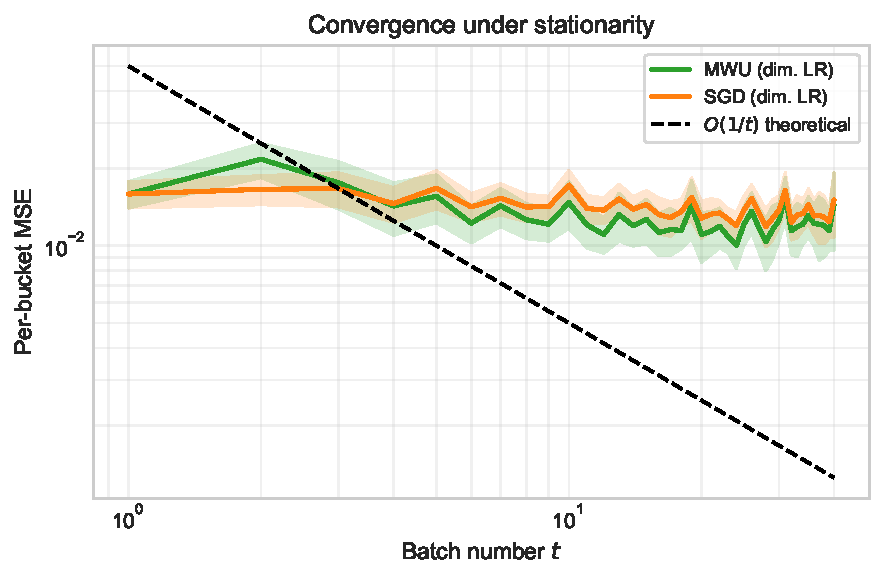
\includegraphics[width=0.8\textwidth]{figures/convergence_loglog.pdf}
\caption{Log-log plot of per-bucket MSE of calibration error versus batch number under stationarity. Theorem~\ref{thm:convergence} predicts slope $-1$. MWU with diminishing step sizes closely tracks the theoretical $O(1/t)$ rate.}
\label{fig:convergence}
\end{figure}

\subsection{Tracking and Step Size}

Under the linear drift synthetic scenario, Figure~\ref{fig:tracking} plots the time-averaged tracking error $\frac{1}{T}\sum_t \frac{1}{B}\sum_b (\ell_b^{(t)})^2$ as a function of the constant step size $\eta$, for $\eta \in \{0.001, 0.005, 0.01, 0.05, 0.1, 0.5, 1.0, 2.0\}$. Theorem~\ref{thm:tracking} predicts a U-shape: small $\eta$ incurs tracking lag (bias term dominates), large $\eta$ incurs noise (variance term dominates). We overlay the theoretical bound with estimated $\sigma^2$, $\mu$, and $V_T$.

\begin{figure}[t]
\centering
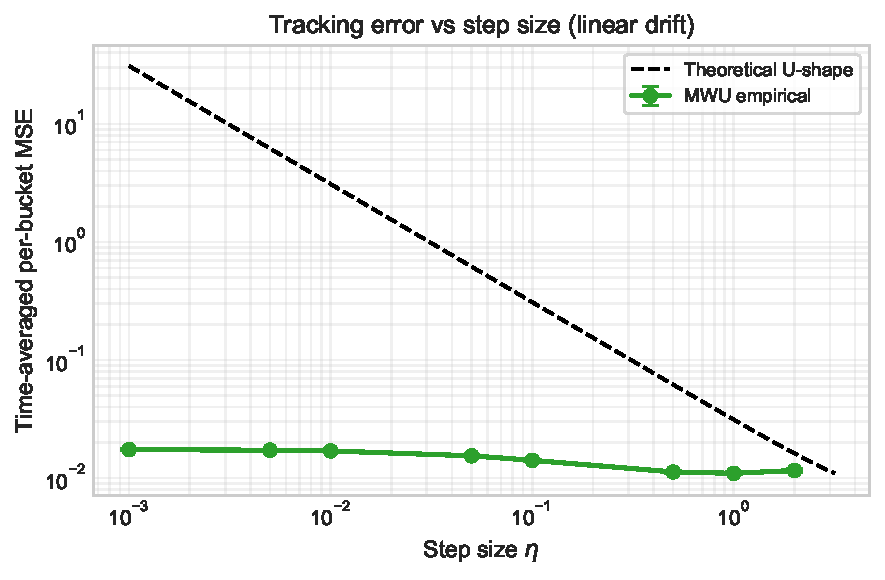
\includegraphics[width=0.8\textwidth]{figures/tracking_eta.pdf}
\caption{Time-averaged calibration error versus step size $\eta$ under linear drift. The empirical curve exhibits the U-shape predicted by Theorem~\ref{thm:tracking}: small $\eta$ incurs tracking lag, large $\eta$ incurs noise.}
\label{fig:tracking}
\end{figure}

Under the sudden-shift scenario, Figure~\ref{fig:recovery} plots ECE as a time series for all methods. MWU and EMA should adapt within one or two batches. Platt retrained every 10 batches will lag by up to 10 batches. Isotonic retrained every batch should recover at the next refit. We report time-to-recovery for each method.

\begin{figure}[t]
\centering
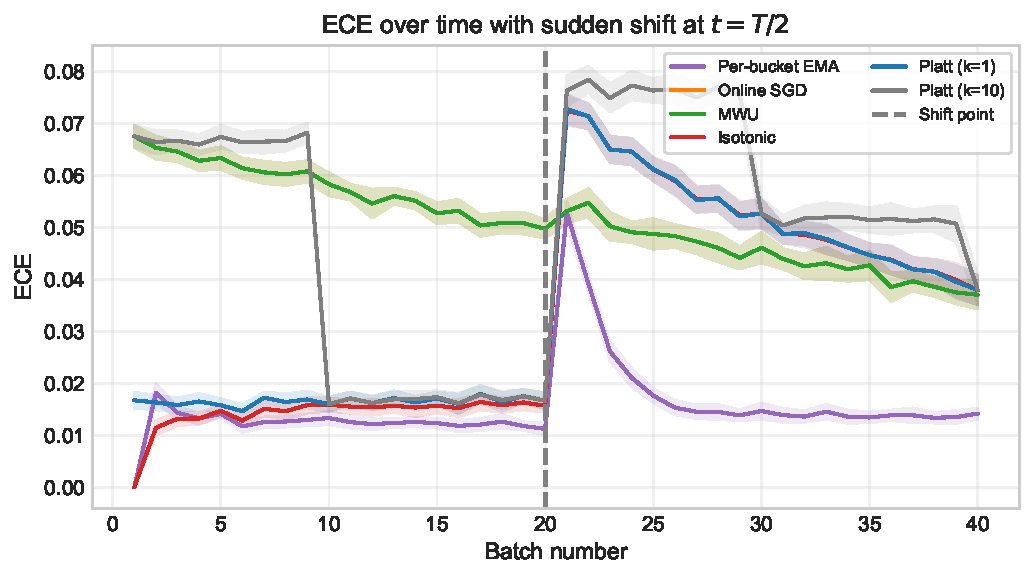
\includegraphics[width=0.8\textwidth]{figures/recovery.pdf}
\caption{ECE over time under sudden shift at $t = T/2$. Streaming methods (MWU, EMA, SGD) adapt within 1--2 batches after the shift. Batch methods that refit frequently (Platt $k=1$, Isotonic) also recover quickly, while Platt with $k=10$ lags by several batches.}
\label{fig:recovery}
\end{figure}

Table~\ref{tab:drift_scenarios} summarizes final ECE across all six drift scenarios on the synthetic stream. Per-bucket EMA achieves the lowest ECE across scenarios by directly tracking outcome rates, though it sacrifices within-bucket discrimination. MWU and Online SGD, which preserve the raw model's ordering within buckets, perform comparably and show particular strength under the sudden-shift scenario where rapid adaptation matters.

\begin{table}[H]
\centering
\begin{tabular}{@{}lccccc@{}}
\toprule
Scenario & Platt & Isotonic & MWU & EMA & SGD\\
\midrule
Stationary & 0.0172 & 0.0172 & 0.0422 & 0.0127 & 0.0422\\
Linear Up & 0.0539 & 0.0540 & 0.0520 & 0.0149 & 0.0520\\
Linear Down & 0.0545 & 0.0546 & 0.0594 & 0.0146 & 0.0594\\
Sinusoidal & 0.0196 & 0.0195 & 0.0451 & 0.0160 & 0.0451\\
Sudden Shift & 0.0380 & 0.0379 & 0.0371 & 0.0142 & 0.0371\\
Random Walk & 0.0250 & 0.0243 & 0.0480 & 0.0132 & 0.0480\\
\bottomrule
\end{tabular}
\caption{Final ECE by drift scenario (synthetic stream, $B=100$, 20 seeds). Lower is better. EMA achieves lowest ECE by tracking bucket outcome rates directly, while MWU and SGD preserve within-bucket discrimination from the raw model.}
\label{tab:drift_scenarios}
\end{table}

\subsection{Sensitivity to Bucketing and Batch Size}

The theory predicts that MWU's performance degrades when bucket-level noise is large (small $n_b$) and when the strong monotonicity constant $\mu$ is small (extreme buckets). We test both.

\paragraph{Number of buckets.} We vary $B \in \{10, 25, 50, 100, 200\}$ on the semi-synthetic streams, holding batch size fixed at 2,000. With $B = 200$ and 2,000 observations per batch, the average bucket contains only 10 observations, making $\ell_b$ a noisy estimate. We expect MWU and EMA to degrade at large $B$, while batch methods (which pool across all historical data) should be more robust.

\paragraph{Batch size.} We vary batch size in $\{200, 500, 1000, 2000, 5000\}$ with $B = 50$ fixed. Smaller batches mean noisier per-bucket estimates ($\sigma^2$ grows) and more frequent updates. Theorem~\ref{thm:tracking} predicts that the variance term $\eta\sigma^2/\mu$ grows, requiring smaller $\eta$ to compensate. We report how each method's ECE changes with batch size.

\paragraph{Per-bucket analysis.} On the semi-synthetic streams, we report calibration error separately for buckets in the bottom decile ($p^{\mathrm{raw}} < 0.1$), middle deciles ($0.3 < p^{\mathrm{raw}} < 0.7$), and top decile ($p^{\mathrm{raw}} > 0.9$) of the raw probability distribution. The condition number remark following Theorem~\ref{thm:convergence} predicts that MWU converges fastest in the middle and slowest at the extremes, because $q(1-q)$ is largest near $q = 0.5$. EMA, which does not use the odds-ratio structure, should not exhibit this pattern.

\subsection{Scaling}

On the production-scale simulation (10M impressions, 1,000 batches), we report wall-clock time per batch as a function of cumulative data volume. MWU and EMA should be flat (constant time per batch). Batch methods retrained on all historical data should grow linearly. Platt retrained on a sliding window of fixed size provides an intermediate point.

\begin{figure}[t]
\centering
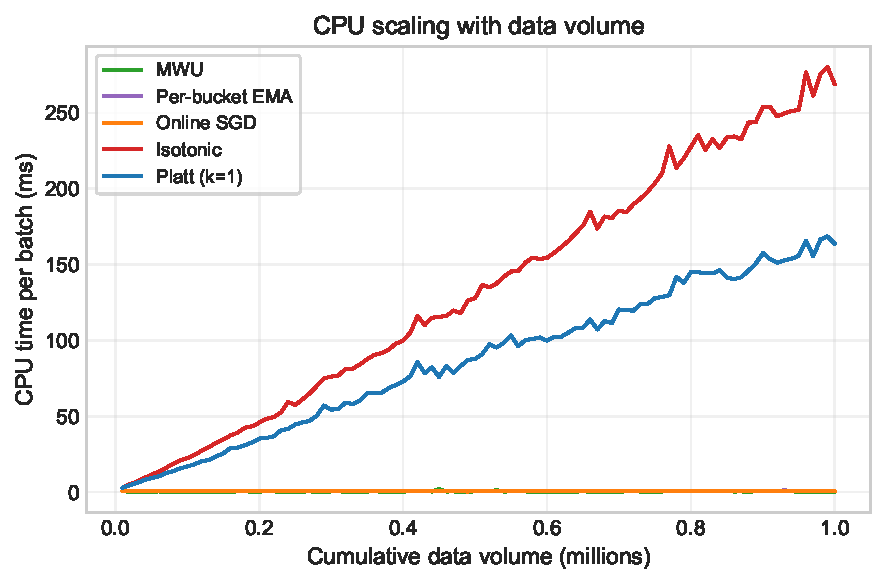
\includegraphics[width=0.8\textwidth]{figures/scaling.pdf}
\caption{CPU time per batch versus cumulative data volume (1M impressions, 100 batches). MWU and EMA maintain constant time per batch while batch methods (Isotonic, Platt) grow linearly with data volume.}
\label{fig:scaling}
\end{figure}

\section{Discussion}
\label{sec:discussion}

The theoretical analysis reveals that the MWU calibrator's effectiveness is not incidental. The derivative of the calibration map with respect to the log-bias factor is $q(1-q)$, the Bernoulli variance of the calibrated prediction. This makes the calibration map a strictly monotone operator: overprediction in a bucket generates a restoring force that pushes the bias factor down, and underprediction generates a force that pushes it up. The self-correcting structure is what makes simple root-finding (Robbins-Monro) work, and why convergence is faster ($O(1/t)$) than what generic regret bounds provide ($O(1/\sqrt{T})$).

Theorem~\ref{thm:tracking} gives practitioners a concrete knob: the step size $\eta$ controls the bias-variance tradeoff between tracking lag and noise sensitivity. The optimal step size depends on the drift rate, which is unknown, but the bound suggests a heuristic: increase $\eta$ when the calibration error is persistently signed (indicating drift), decrease it when errors oscillate around zero (indicating stationarity). An adaptive step size that implements this logic automatically is a natural next step.

The approach is most useful when data arrive continuously and calibration must track drift without expensive refits, as in ad bidding, real-time risk scoring, and clinical triage under changing patient populations. It is less useful when the raw model's bucketing is poorly chosen (miscalibration within buckets cannot be corrected by per-bucket bias factors) or when the number of buckets $B$ is very large relative to batch size (insufficient observations per bucket to estimate $\ell_b$ reliably).

\section{Conclusion}
\label{sec:conclusion}

We analyzed the multiplicative-weights calibrator as a Robbins-Monro stochastic approximation scheme, showing that the calibration map is a strongly monotone operator with Bernoulli-variance curvature. This yields $O(1/t)$ convergence of the actual calibration error under stationarity and explicit tracking bounds under drift. The per-batch update is a single exponential step per bucket, matches the accuracy of batch calibrators, adapts faster to distributional shifts, and requires two orders of magnitude less compute.

\bibliographystyle{apalike}
\bibliography{mwu}

\end{document}